\chapter{Marco Te\'orico}
\section{El Lenguaje}
En un contexto general el lenguaje es un sistema de comunicaci\'on que todo ser vivo 
utiliza para intercambiar informaci\'on con sus semejantes mediante el uso de
s\'imbolos, se\~nales y sonidos percibidos por los \'organos sensoriales. \\

El principal tipo lenguaje utilizado por el ser humano es el \emph{Lenguaje Natural}, 
adem\'as se han desarrollado otros tipos de lenguajes para su comunicaci\'on como ser 
el lenguaje braille y el lenguaje de se\~nas, que son utilizados en ausencia de 
capacidades para utilizar un lenguaje natural. \\

Otros tipos de lenguajes existentes son los \emph{lenguajes formales}, que
son construcci\'ones artificiales, donde los s\'imbolos y reglas para unir los mismos
est\'an formalmente especificados, los lenguajes de programaci\'on utilizados en 
inform\'atica son un ejemplo de lenguaje formal.


\section{Lenguaje Natural}
Las capacidades humanas de comunicaci\'on se basan en el uso de signos ling\"uisticos
que se componen por un concepto (\emph{significado}) y una imagen ac\'ustica
(\emph{significante}), cuando estos signos se asocian a una sintaxis generan  una
\emph{lengua natural}, el uso de estas lenguas describen un lenguaje natural. \\

Los idiomas como ser el espa\~nol o el ingl\'es, al contar con un conjunto de signos
(\emph{alfabeto}) y reglas sint\'acticas (\emph{gram\'atica}) propias para cada uno,
representan lenguajes naturales.

\subsection{Alfabeto}
Es el conjunto de simbolos utilizados en un idioma para representar estructuras del
lenguaje como las palabras.

\subsection{Gram\'atica}
Es el conjunto de reglas que gobiernan la composici\'on de las palabras dentro de un
lenguaje natural.


\section{La Palabra}
La Palabra es la unidad m\'inima con significado que se puede pronunciar de manera
aislada (evidencia fonol\'ogica)\cite{HOET09}. La rama de la ling\"uistica que estudia
la composici\'on y estructura interna de las palabras es la morfolog\'ia.

\subsection{Clasificaci\'on de las palabras}
La clasificaci\'on de las palabras se puede hacer en funci\'on de diferentes criterios:
categor\'ia gramatical, estructura interna, acentuaci\'on y n\'umero de s\'ilabas. \\

La clasificaci\'on por categor\'ia gramatical es la siguiente:

\begin{description}[leftmargin=0cm]
	\item{Sustantivo} Cualquier abstracci\'on o entidad concreta, una 
	persona (\emph{Maria}), lugar (\emph{La Paz}) o idea (\emph{felicidad}).
	\item[Verbo] Cualquier acci\'on (\emph{caminar}) u ocurrencia (\emph{sucedi\'o}).
	\item[Adjetivo] Cualquier calificador del sustantivo (\emph{grande}).
	\item[Adverbio] Cualquier calificador de un adjetivo, verbo u otro
	adverbio (\emph{muy}).
	\item[Determinante] Cualquiera que precise un sustantivo (\emph{el}).
	\item[Preposici\'on] Cualquiera que establezca una relaci'on y contexto sint\'actico
	(\emph{en}).
	\item[Conjunci\'on] Cualquier conector sint\'actico (\emph{y}).
	\item[Pronombre] Cualquier sustituto de un sustantivo (\emph{alg\'un}).
	\item[Interjecci\'on] Cualquier expresi\'on emocional (\emph{Ahy!}).
\end{description}


\section{Procesamiento del Lenguaje Natural}
El Procesamiento del Lenguaje Natural (PLN) es un campo de la inform\'atica y la 
ling\"uistica concerniente con la interacci\'on entre computadoras y lenguajes
humanos. \\

La interacci\'on se produce con la \emph{generaci\'on} de lenguaje legible por humanos
a partir de datos procesados y la \emph{comprensi\'on} del lenguaje humano para su
representaci\'on formal.


\section{Etiquetado gramatical}
Es la acci\'on de asignar a cada palabra una \emph{etiqueta} que describe como es
utilizada esta palabra en un texto dado. Tipicamente estas etiquetas indican una
sintactica, y ocasionalmente incluyen informaci\'on caracter\'istica adicional, tal
como ser g\'enero (masculino o femenio) o la conjugaci\'on verbal \cite{TH99}. \\

Su principal dificultad radica en la ambig\"uedad inherente
que tienen las palabras, por ejemplo la palabra \emph{llama} puede hacer referencia a 
un animal, en este caso es un sustantivo pero tambi\'en puede hacer referencia al 
acto de realizar una llamada telef\'onica, en este otro caso es un
verbo, para hacer frente a esta dificultad los algoritmos de etiquetado gramatical 
deben tomar en cuenta el contexto de las palabras, generalmente haciendo uso de un 
\emph{Corpus Ling\"uistico}). \\

Existen varios m\'etodos para el etiquedo gramatical: basado en \emph{Modelo Oculto
de Markov}, basados en sistemas expertos, basados en modelos de lenguaje como
\emph{Modelo de M\'axima Entropia} o \emph{Modelo N-gram}. \\

En el presente trabajo se utilizar el m\'etodo basado en el Modelo Oculto de Markov.

\subsection{Modelo Oculto de Markov}
Un Modelo Oculto de Markov (MOM) es una construcci\'on estad\'istica que puede ser
utilizada para resolver problemas de clasificaci\'on que tengan una representaci\'on
por secuencia de estados. Estos estados estan conectados por un conjunto
de \emph{probabilidades de transici\'on}, los cuales indican la probabilidad de pasar
entre dos estados dados. Un proceso inicia en alg\'un estado, entonces en intervalos
discretos de tiempo, el proceso se mueve a un nuevo estado seg\'un lo indicado 
por las probabilidades de transici\'on. En un MOM, la secuencia exacta de estados
que el proceso genera son desconocidos (ocultos). Cuando el proceso entra en cada
estado, se elige un \emph{s\'imbolo de salida} con una distribuci\'on de probabilidad
espec\'ifica para cada uno, La salida de MOM es una secuencia de simbolos de 
salida \cite{TH99}. \\

Seg\'un Rabiner \cite{TH99} se necesitan 5 elementos para definir un MOM:
\begin{enumerate}
	\item \emph{N}, el n\'umero de estados distintos en el modelo. Para el etiquetado
	gramatical, \emph{N} es el n\'umero de etiquetas gramaticales que son utilizadas 
	por el sistema. Cada etiqueta corresponde a un estado del MOM.
	\item \emph{M}, el n\'umero de distintos s\'imbolos de salida en el alfabeto del
	MOM. Para el etiquetado gramatical, \emph{M} es el n\'umero de palabras del
	l\'exico utilizado por el sistema.
	\item $A = \{a_{ij}\}$, la probabilidad de transici\'on de pasar del estado $i$ al 
	estado $j$.  Para el etiquetado gramatical,  $a_{ij}$ representa  la probabilidad de 
	pasar de la etiqueta $t_i$ a la etiqueta $t_j$, en otras palabras es la probabilidad
	que la etiqueta $t_j$ se encuentre despu\'es de la etiqueta $t_i$, por ejemplo
	la probabilidad que un verbo este despu\'es de un determinante; la estimaci\'on
	de esta probabilidad se obtiene a partir del corpus utilizado.
	\item $B=\{b_j(k)\}$, la distribuci\'on de probabilidad de los simbolos bajo
	observaci\'on, $b_j(k)$ es la probabilidad que el k-\'esimo simbolo de salidad sea 
	elegido cuando el modelo se encuentra en el estado $j$. Para el etiquetado 
	gramatical, es la probabilidad que la palabra $w_k$ sea elegida cuando el sistema se 
	encuentre en la etiqueta $t_j$ ($P(w_k|t_j)$); la estimaci\'on de esta probabilidad
	se obtiene a partir del corpus utilizado.
	\item $\pi = \{\pi_i\}$, la distribuci\'on inicial de estados, $\pi_i$ es la
	probabilidad que el modelo inicie en el estado $i$. Para el etiquetado gramatical,
	es la probabilidad que el texto inicie con la etiqueda $t_i$.
\end{enumerate}

Cuando se utiliza el MOM para el etiquetado gramatical, el objetivo es determinar
la secuencia mas probable de etiqueta (estados) que generan la palabras en el texto
(secuencia de simbolos de salida). En otras palabras, dado un texto $V$, calcular
la secuencia $U$ de etiquetas que maximize $P(V|U)$.\\

El algoritmo \emph{Viterbi} es un m\'etodo usual para calcular la secuencia m\'as
probable de etiquetas cuando se utiliza un MOM.



\section{Selecci\'on de palabras clave}
Las palabras clave se definen como una secuencia de una o mas palabras que idealmente
proveen una representaci\'on compacta de la esencia del contenido de un 
documento \cite{REC10}. \\

Las palabras clave se utilizan para catalogar e indexar material bibliogr\'afico,
su identificaci\'on es una de las tareas principales en el procesamiento de texto. \\

La asignaci\'on manual de palabras claves de calidad es costosa, consume tiempo y es
propensa a error, por lo tanto se han propuesto varios m\'etodos para su seleccio\'on
autom\'atica.

\subsection{M\'etodos de selecci\'on de palabras clave}
Los m\'etodos de selecci\'on de palabras claves se dividen en cuatro categor\'ias:
estad\'isticas simples, ling\"uisticos, aprendizaje autom\'atico y otros \cite{ZWW08}.
\begin{description}[leftmargin=0cm]
	\item[Enfoques estad\'isticos] Son los mas simples, no necesitan datos previos,
	la informaci\'on estad\'istica de las palabras pueden ser usadas para identificar
	las palabras clave en un documento.
	\item[Enfoques ling\"uisticos] Utilizan las caracter\'isticas l\'exicas y
	sint\'acticas de las palabras, sentencias y documentos.
	\item[Enfoques de aprendizaje autom\'atico] Se basan en el aprendizaje supervisado
	a partir de datos de ejemplo para generar un modelo y aplicarlo a nuevos
	documentos.
	\item[Otros enfoques] Combinan los m\'etodos anteriormente mencionados o utilizan
	conocimiento heur\'istico.
\end{description}

\section{Modelo TextRank}
Es un m\'odelo de puntuaci\'on basado en grafos para el procesamiento de
texto \cite{RMPT04}, que es utilizado para la extracci\'on de palabras claves
y sentencias mediante algoritmos de puntuaci\'on basados en grafos.
% TODO: Completar este concepto

\subsection{Algoritmos de puntuaci\'on basados en grafos}
Son algoritmos que se utilizan para obtener valores significativos
(\emph{calificaci\'on}) de los nodos en un grafo. \\

Existen varios algoritmos de puntuaci\'on: \emph{PageRank} de Google,
\emph{HITS} de Kleinberg, \emph{Positional Function} de Herings \cite{RM04}. \\

A continuaci\'on se describe el algoritmo PageRank.

\subsubsection{Algoritmo PageRank}
\begin{figure}
	\centering
		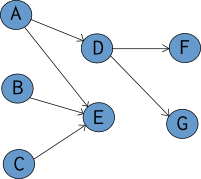
\includegraphics[]{recursos/img/grafoDirigido.png}
		\caption {Grafo dirigido}
\end{figure}

Dado $G=(V,E)$ un grafo dirigido, con un conjunto de v\'ertices $V$ y un conjunto
de arcos $E$, donde $E$ es un subconjunto de $V x V$, llamamos $In(V_i)$ al
conjunto de v\'ertices que apuntan a $V_i$ (predecesores),  en la Figura 2.1
$In(E)=\{A,B,C\}$, y $Out(V_i)$ al conjunto de v\'ertices que son apuntados por $(V_i)$
(sucesores), en la Figura 2.1 $Out(D)=\{F,G\}$ . El puntaje del v\'ertice $V_i$ 
esta dado por \cite{SBLP98}:

\begin{equation}
	S(V_i) = (1 - d) + d * \sum_{V_j\in In(V_i)}{\frac{1}{|Out(V_j)|}S(V_j)}
\end{equation}

donde $d$ es un factor de amortiguaci\'on que toma valores comprendidos entre
0 y 1, que expresa la probabilidad de avanzar de un v\'ertice a otro de manera
aleatoria, generalmente tiene el valor de 0.85 \cite{SBLP98}.

\subsection{Aplicaci\'on en la extracci\'on de palabras claves}
El grafo es construido de la siguiente manera: se seleccionan palabras  para 
conformar los v\'ertices, si existe una relaci\'on de \emph{co-ocurrencia} entre 
las palabras seleccionadas, se a\~nade un nodo entre ellas. \\

Las palabras seleccionadas son aquellas que pasan por un filtro sint\'actico, el cual
selecciona solo las unidades l\'exicas pertenecientes a un conjunto definido de tipos
de palabras. \\

Se pueden seleccionar todos los tipos de palabras, o un conjunto restringido a verbos
y sustantivos, se presentan mejores resultados con el conjunto de verbos y
adjetivos \cite{RMPT04} .
